\section{Count and Probability Matrices}
\begin{frame}{Count and Probability Matrices}
    \textbf{Count Matrix:} A matrix that counts occurrences of word pairs in a corpus.
    
    \vspace{1em}
    \textbf{Probability Matrix:} A matrix that calculates probabilities of word pairs based on counts.
    
    \vspace{1em}
    \textbf{Example:} For the sentence "I love NLP. I love AI."
    \begin{itemize}
        \item Count Matrix: Counts how many times each word appears with every other word.
        \item Probability Matrix: Calculates the probability of each word appearing given the previous word.
    \end{itemize}
\end{frame}

\begin{frame}{Count Matrix}
    \begin{figure}
        \centering
        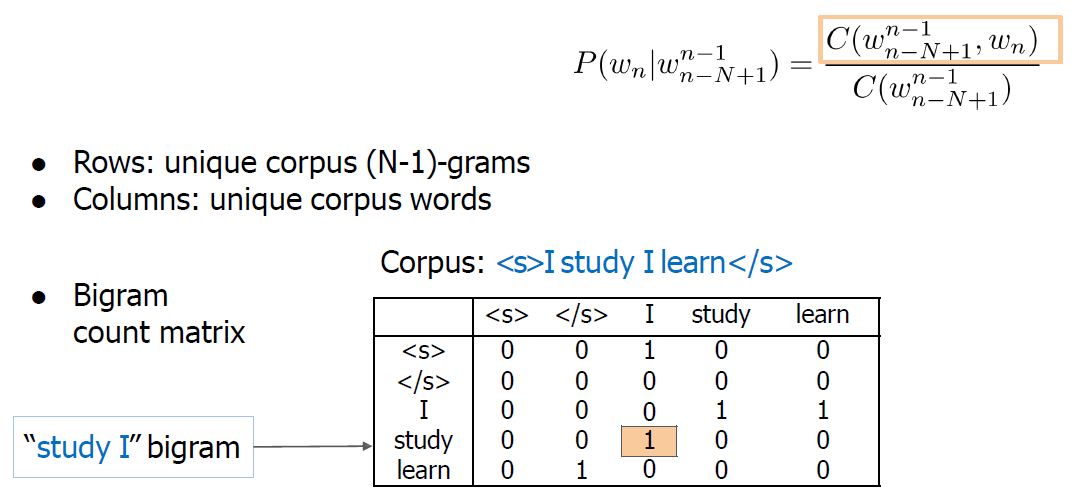
\includegraphics[height=0.8\textheight,width=1\textwidth,keepaspectratio]{images/nlp-intro/count-matrix.png}
    \end{figure}
\end{frame}

\begin{frame}{Count Matrix Example}
    \textbf{Text:} "I love NLP. I love AI."
    
    \vspace{1em}
    \textbf{Bigrams:}
    \begin{itemize}
        \item (I, love): 2
        \item (love, NLP): 1
        \item (love, AI): 1
    \end{itemize}
    
    \vspace{1em}
    \textbf{Count Matrix:}
    \begin{itemize}
        \item Rows: Words in the corpus
        \item Columns: Words in the corpus
        \item Cells: Count of occurrences of each word pair
    \end{itemize}
\end{frame}

\begin{frame}{Probability Matrix}
    \begin{figure}
        \centering
        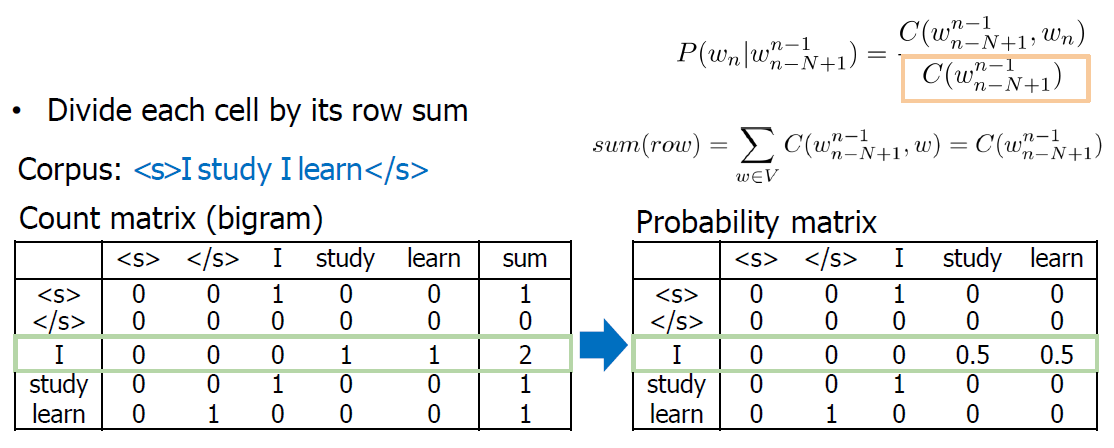
\includegraphics[height=0.8\textheight,width=1\textwidth,keepaspectratio]{images/nlp-intro/probability-matrix.png}
    \end{figure}
\end{frame}

\begin{frame}{Probability Matrix Example}
    \textbf{Probability Calculation:}
    
    \vspace{1em}
    \textbf{Bigram Probability:}
    \[
        P(\text{love} \mid \text{I}) = \frac{\text{Count}(\text{I}, \text{love})}{\text{Count}(\text{I})} = \frac{2}{2} = 1
    \]
    
    \vspace{1em}
    \textbf{Probability Matrix:}
    \begin{itemize}
        \item Rows: Words in the corpus
        \item Columns: Words in the corpus
        \item Cells: Probability of each word given the previous word
    \end{itemize}
\end{frame}
